\documentclass[a4paper,12pt]{article}
\usepackage[latin1]{inputenc}
\usepackage[spanish]{babel}
\usepackage{bm}
\usepackage{graphicx}
\usepackage{amsmath}
\setlength{\textheight}{235mm}
\setlength{\textwidth}{168mm}
\setlength{\oddsidemargin}{0pt}
\pagestyle{empty}
\begin{document}
\mbox{}\vspace*{-45mm}

{\centering
{\small\sc Escuela T�cnica Superior de Ingenieros de Caminos, Canales y
Puertos (Madrid)}\\*[4mm]
{\Large\bf M�todo de los Elementos Finitos}\\*[4mm]
Ejercicio 3: Elasticidad lineal \\*[4mm]

}

\vspace{3mm}

%%%%%
\parbox{0.50\textwidth}{
Se considera una viga en m�nsula con las dimensiones y geometr�a indicadas
en la figura. En el extremo libre act�a una carga vertical descendente
$P=10$ kN. El m�dulo el�stico es $E=20$ GPa y el coeficiente de Poison
$\nu=0$. Se considerar� la hip�tesis correspondiente a tensi�n plana, con
un espesor $t=1$ m.

Para resolver el correspondiente modelo de elementos finitos, con el
programa {\tt FEAP},  se considerar�
una malla con $11 \times 3$ {\em nodos}, discretizada con elementos
cuadril�teros de $4$ y $8$ nodos, y elementos triangulares de $3$ y $6$ nodos.
}\hfill
\parbox{0.50\textwidth}{ \hfill
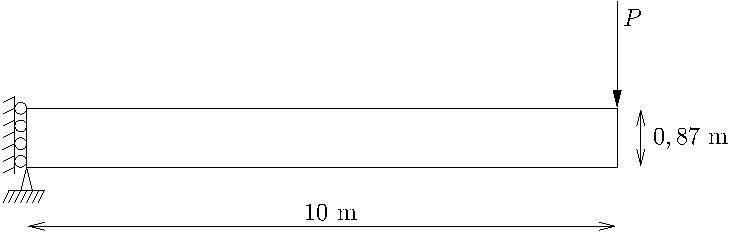
\includegraphics[width=0.5\textwidth]{ejercicio3}
}
\\

{\bf NOTAS:}
\begin{enumerate}

\item La malla se generar� con la instrucci�n {\tt block}, tomando las
esquinas en el orden indicado en la siguiente figura.
\item Los elementos triangulares tendr�n la hipotenusa en la direcci�n
$1-3$ de las esquinas del bloque.
\item La f�rmula de Resistencia de Materiales que permite calcular la
flecha en el extremo es: $f=\frac{1}{3} \frac{PL^3}{EI}$.
\item {\em Se cargar� el fichero postscipt de contornos de movimientos en direcci�n vertical para la malla de elementos cuadril�teros de 4 nodos}
\end{enumerate}
\begin{center}
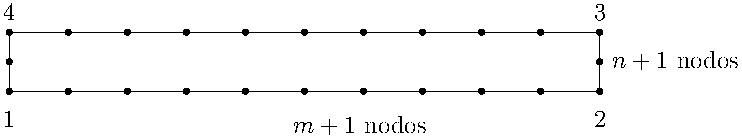
\includegraphics[width=0.60\textwidth]{bloque3}
\end{center}
\end{document}
